\chapter{\label{cap:antecedentes}Antecedentes}

Uno de los propósitos principales del laboratorio de Óptica Cuántica de Rydberg es generar estados no clásicos de luz con átomos de Rydberg, para lograr esto necesitamos de un medio no lineal y analizar la luz que sale de tal medio. En nuestro caso, la no linealidad del medio atómico la obtendremos con el fenómeno de \textbf{Transparencia Electromagnéticamente Inducida} (EIT, por sus siglas en inglés), y mediante \textbf{átomos de Rydberg} incrementaremos las no linealidades. En este capítulo presento brevemente la bases teóricas de EIT, un poco sobre átomos de Rydberg y de óptica cuántica no lineal\miNota{a i a i a i a i a i a i a i a i a i a i a i a i a i a i a i a i a i a i a i a i a i }.

\section{\label{sec:interaccionLuzMateria}Interacción luz-materia}

Gracias a las contribuciones de Planck y la evidencia experimental sobre el comportamiento de la materia sabemos que la energía de los electrones ligados a los átomos es discreta, no pueden adquirir un valor arbitrario de energía como sí lo hacen los electrones libres. Y aún así estos valores discretos o cuantizados, llamados \emph{niveles de energía}, son infinitos. Posteriormente, Schrödinger y contemporáneos proporcionaron las herramientas para resolver y explicar muchas de las observaciones físicas de su época. Si supones que $\phi_\sm{n}(\vektor{r})$ son las funciones propias del Hamiltoniano $\iH_\sm{0}$ para un átomo libre de cualquier campo, entonces la función de onda $\Psi(\vektor{r},t)$ de dicho átomo interactuando con un campo de radiación puede expandir como

\begin{equation}
\label{ec:funcionOndaExpansion}
\Psi(\vektor{r},t)=\sum_{k}c_\sm{k}(t)\phi_\sm{k}(\vektor{r})e^{-j\omega_{k}t}.
\end{equation}

De donde podemos obtener la ecuación de Schrödinger para un átomo interactuando con un campo de radiación~\cite{metcalf}

\begin{equation}
\label{ec:ecuacionSchrodinger}
j\hbar\dfrac{dc_\sm{k}(t)}{dt}= \sum_{l}c_\sm{l}(t)\iH'_\sm{kl}e^{j(\omega_{k}-\omega_{l})t},
\end{equation}

siendo $j$ la unida imaginaria,  $\iH=\iH_\sm{0}+\iH'$ el Hamiltoniano total del sistema y $\iH'_{kl}$ los elementos de matriz del Hamiltoniano de interacción entre el campo y el átomo $\iH'$. Sin embargo, resolver analíticamente la anterior ecuación es imposible, a pesar de que estamos tratando con un solo átomo. Por ello es necesario realizar aproximaciones o simulaciones numéricas.

\subsection{\label{sub:atomo2Niveles}Átomo de dos niveles}

\p Una de los métodos más famosos para tratar la interacción de la luz con un átomo se lo debemos a Rabi~\cite{rabi}, el \textbf{átomo de dos niveles}. Este modelo aborda el problema en un espacio de Hilbert de dimensión reducida, en concreto, uno generado por una base de tan solo dos elementos. Dicha aproximación es válida siempre que las transiciones a otros niveles de energía del átomo sean despreciables y no participan en la dinámica de la interacción. Gracias a este modelo semiclásico podemos explicar diversos comportamientos, tales como las oscilaciones de Rabi, estados vestidos, enfriamiento láser, fluorescencia e incluso la consistencia con otras teorías clásicas, como el modelo de Lorentz (un átomo cuyo electrón está ligado como un oscilador armónico amortiguado) o los coeficientes $A$ y $B$ de Einstein en sus ecuaciones de población de los niveles de energía~\cite{steck2}.

\subsection{\label{sub:atomo3Niveles}Átomo de tres niveles}

\p El siguiente paso de complejidad, al menos en lo que este proyecto respecta, es aumentar a tres la dimensión del espacio de Hilbert, esto es, un \textbf{átomo de tres niveles}. En nuestro caso tenemos dos campos interactuando con el átomo, correspondientes a los láseres que acoplan sus niveles. La especie atómica que utilizamos en los experimentos es rubidio~\cite{rb85,rb87}, los tres estados que están considerados son el estado base $\ket{g}:5\prescript{2}{}{\mathrm{S}}_\sm{1/2}$, el primer estado excitado $\ket{e}:5\prescript{2}{}{\mathrm{P}}_\sm{3/2}$ y otro estado excitado $\ket{r}:n\mathrm{S}$ o $n\mathrm{D}$ según las reglas de selección de transición dipolar. Un láser acopla el estado base con el primer estado excitado y que denominamos láser o \emph{haz de prueba}, el segundo láser va desde el primer estado excitado al otro estado excitado y llamamos \emph{haz de control}, de manera que la configuración de niveles relevantes es la \emph{configuración escalera} (fig.~\ref{fig:configuraciones}). 

\begin{figure}[H]
\centering
\begin{minipage}{0.8\textwidth}
\centering
\includegraphics[width=0.875\textwidth]{configuraciones}
\caption{\label{fig:configuraciones}Configuraciones en las que un átomo de tres niveles puede interactuar con el campo de dos haces láser. De izquierda a derecha son las configuraciones escalera, $\Lambda$ y V. Las energías $\hbar\omega_{1}$ y $\hbar\omega_{2}$ son las energías de transición naturales del átomo, mientras que las frecuencias angulares $\omega_{p}$ y $\omega_{c}$ representan a los láseres de prueba y control, respectivamente. Además, $\Delta_{1}$ y $\Delta_{2}$ son las desintonías netas de la frecuencia de un láser respecto a la frecuencia natural de la transición atómica.}
\end{minipage}
\end{figure}

Bajo las anteriores consideraciones, el Hamiltoniano de este sistema, un átomo de tres niveles interactuando con dos campos de radiación, es $\iH=\iH_\sm{\mathrm{a}}+\iH_\sm{\mathrm{int}}$ donde

\begin{equation}
\label{ec:hamiltonianoAtomico}
\iH_\sm{\mathrm{a}}=\dfrac{\hat{\vektor{P}}^{2}}{2m}+\hbar\omega_\sm{1}\hat{\sigma}_\sm{ee}+\hbar\left(\omega_\sm{1}+\omega_\sm{2}\right)\hat{\sigma}_\sm{rr},
\end{equation}

\begin{equation}
\label{ec:hamiltonianoInteraccion}
\begin{split}
\iH_\sm{\mathrm{int}}= & \hspace{1mm}\dfrac{\hbar}{2}\left[\Omega^{*}_\sm{p}(\vektor{r})e^{-j\left(\vektor{k}_{p}\cdot\vektor{r}-\omega_{p}t\right)}\hat{\sigma}_\sm{ge}+\Omega_\sm{p}(\vektor{r})e^{j\left(\vektor{k}_{p}\cdot\vektor{r}-\omega_{p}t\right)}\hat{\sigma}_\sm{ge}^{\dagger}\right]+\\
& \hspace{1mm}\dfrac{\hbar}{2}\left[\Omega^{*}_\sm{c}(\vektor{r})e^{-j\left(\vektor{k}_{c}\cdot\vektor{r}-\omega_{c}t\right)}\hat{\sigma}_\sm{er}+\Omega_\sm{c}(\vektor{r})e^{j\left(\vektor{k}_{c}\cdot\vektor{r}-\omega_{c}t\right)}\hat{\sigma}_\sm{er}^{\dagger}\right],
\end{split}
\end{equation}

siendo $\omega_\sm{1,2}$ las frecuencias angulares de transición naturales del átomo, $\omega_\sm{p,c}$ las frecuencias angulares de los láseres, $\sigma_{ab}\coloneqq\ketbra{a}{b}$ son operadores de descenso y las frecuencias de Rabi dadas por

\begin{equation}
\label{ec:frecuenciasRabi}
\Omega_\sm{x}(\vektor{r})=\dfrac{\abs{d_\sm{x}}}{\hbar}E_\sm{x}(\vektor{r})e^{j\phi_{x}(\vektor{r})},
\end{equation}

donde $d_\sm{x}$ es el elemento de matriz del operador dipolar atómico $\hat{\vektor{d}}$ correspondiente a la transición acoplada por el campo con intensidad $E_\sm{x}$ y fase $\phi_\sm{x}$. Para incluir procesos no unitarios como el decaimiento espontáneo y decoherencias utilizamos el formalismo de la \emph{matriz de densidad} $\rho$, así la ecuación maestra que rige la dinámica del sistema es

\begin{equation}
\label{ec:ecuacionMaestra}
\dfrac{\partial\tilde{\rho}}{\partial t}=-\dfrac{j}{\hbar}\left[\tilde{\iH},\tilde{\rho}\right]+\Gamma_\sm{e}\D[\hat{\sigma}_\sm{ge}]\hat{\rho}+\Gamma_\sm{r}\D[\hat{\sigma}_\sm{er}]\hat{\rho}+\gamma_\sm{g}\D[\hat{\sigma}_\sm{g}]\hat{\rho},
\end{equation}

con $\Gamma_\sm{e}$ la tasa de decaimiento del estado $\ket{e}$ al estado base $\ket{g}$, $\Gamma_\sm{r}$ la tasa de decaimiento del estado $\ket{r}$ al estado $\ket{e}$. El coeficiente $\gamma_\sm{g}$ toma en cuenta todos los procesos de pérdida de coherencia entre los estados, también está el operador $\hat{\sigma}_\sm{g}\coloneqq\ketbra{g}{g}-\ketbra{r}{r}$ y el súper operador Lindbladiano $\D$~\cite{breuer}.

\subsection{\label{sub:eit}Transparencia Electromagnéticamente Inducida}

A partir de la ecuación maestra (ec.~\ref{ec:ecuacionMaestra}) es posible dar con varios resultados de la interacción entre un átomo y dos láseres considerando sólo tres niveles de energía en la dinámica de sus grados de libertad internos. En particular la respuesta óptica de un medio atómico, es decir, cómo reacciona el medio a campos eléctricos externos.

\p Una da las magnitudes o entidades que contiene la información de la susodicha respuesta óptica es la \emph{susceptibilidad eléctrica} $\chi$, que manifiesta cómo se polariza un medio al aplicar un campo eléctrico debido a sus constituyentes atómicos que actúan como dipolos. La relación entre el campo eléctrico aplicado $ \vektor{E}$ y la polarización del medio $\vektor{P}$ está dada por

\begin{equation}
\label{ec:polarizacionCampoE}
\vektor{P}^\sm{(+)}=\epsilon_\sm{0}\chi\vektor{E}^\sm{(+)},
\end{equation}

suponiendo una respuesta lineal del medio al campo aplicado ($\chi$ un escalar) y el superíndice $(+)$ indica la componente de frecuencia positiva de dicha cantidad, $\vektor{A}=\vektor{A}^\sm{(+)}+\vektor{A}^\sm{(-)}$ con $\vektor{A}^\sm{(-)}=(\vektor{A}^\sm{(+)})^{*}$. En la anterior ecuación $\epsilon_\sm{0}$ es la \emph{permitividad eléctrica del vacío}. Puesto que la susceptibilidad eléctrica está relacionada con el índice de refracción \emph{complejo} $n_\sm{\mathrm{ref}}$ a través de $n_\sm{\mathrm{ref}}=\sqrt{1+\chi}$ para un gas atómico, entonces $\chi$ nos permite conocer el perfil de absorción $\Im{(n_\sm{\mathrm{ref}})}$ y el índice de refracción (real) $n_{r}=\Re{(n_\sm{\mathrm{ref}})}$ del medio en presencia de luz. Para escribir la susceptibilidad eléctrica (cantidad macroscópica) en términos de propiedades atómicas que ya hemos visto, como las tasas de decaimiento o frecuencias de Rabi, es útil recordar que la polarización de un ensamble de átomos está relacionada con el operador de \textbf{momento dipolar} $\hat{\vektor{d}}$ de un átomo mediante su valor esperado:

\begin{equation}
\label{ec:polarizacionMomentoDipolar}
\vektor{P}^\sm{(+)}=n\braket{\hat{\vektor{d}}^\sm{(+)}},
\end{equation}

y $n$ la densidad numérica del conjunto. En el átomo de tres niveles y los dos láseres, el operador de momento dipolar toma en cuenta el acoplamiento del estado base $\ket{g}$ al primer estado excitado $\ket{e}$ y del este último al otro estado excitado $\ket{r}$ (configuración escalera). Lo que nos interesa medir experimentalmente es la respuesta del medio al haz de prueba, por tanto en $\braket{\hat{\vektor{d}}}$ solamente consideraremos el elemento $\braket{g|\hat{\vektor{d}}|e}$ de la componente de frecuencia positiva. Así, la susceptibilidad para el haz de prueba interactuando con un átomo de tres niveles en la configuración escalera está dada por

\begin{equation}
\label{ec:susceptibilidad}
\chi=\dfrac{n\braket{g|\varepsilon_\sm{p}\cdot\hat{\vektor{d}}|e}^{2}}{\hbar\epsilon_\sm{0}}\dfrac{\Delta_\sm{2}+j\left(\Gamma_\sm{r}/2+2\gamma_\sm{g}\right)}{\left[\Gamma_\sm{r}/2+2\gamma_\sm{g}-j\Delta_\sm{2}\right]\left[\Gamma_\sm{e}/2+\gamma_\sm{g}/2-j\Delta_\sm{1}\right]+\Omega^{2}_\sm{c}/4},
\end{equation}

donde $\varepsilon_\sm{p}$ es el vector unitario de polarización del haz de prueba. En la anterior ecuación es importante la configuración que se está considerando, en el caso abordado aquí, si $\delta_\sm{p}$ y $\delta_\sm{c}$ son las desintonías de los haces de prueba y control, respectivamente, | $\Delta_\sm{1}=\delta_\sm{p}$ y $\Delta_\sm{2}=\delta_\sm{p}+\delta_\sm{c}$.

\begin{figure}[H]
\centering
\begin{minipage}{0.8\textwidth}
\centering
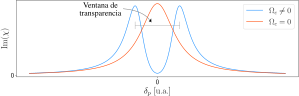
\includegraphics[width=0.875\textwidth]{eit}\\
\includegraphics[width=0.875\textwidth]{dispersion}
\caption{\label{fig:eitDispersion}Las propiedades de un ensamble de átomos se modifican al interactuar con un haz de control resonante. En particular, el medio se vuelve transparente para el haz de prueba en resonancia (gráfica superior) y cambia su índice de refracción (gráfica inferior).}
\end{minipage}
\end{figure}

\p Finalmente, de la ecuación~\ref{ec:susceptibilidad} podemos determinar algunas propiedades macroscópicas. Una de las más interesante emerge cuando el láser de control es resonante con la transición de $\ket{e}$ a $\ket{r}$, es decir, cuando $\delta_\sm{c}=0$ ($\Delta_\sm{1}=\Delta_\sm{2}=\delta_\sm{p}$). En estas condiciones, la interacción del átomo con los campos induce una interferencia entre las vías de excitación, eliminando la absorción en la frecuencia de resonancia de la transición desde $\ket{g}$ a $\ket{e}$. Este fenómeno es la \emph{Transparencia Electromagnéticamente Inducida}~\cite{fleischhauer}, el cual viene acompañado de un medio muy dispersivo~\cite{harris,scully} y que observamos en la figura~\ref{fig:eitDispersion}.

\subsection{\label{sub:luzLenta}Luz lenta}

Que un medio en condiciones de EIT sea altamente dispersivo tiene implicaciones muy interesantes, entre las cuales destaca el cambio en el valor de la velocidad de grupo $v_\sm{g}$ con la cual se propaga un pulso de luz a través de tal medio, velocidad dada por~\cite{harris}	

\begin{equation}
\label{ec:velocidadGrupo}
v_\sm{g}=\dfrac{c}{n_\sm{r}(\omega_\sm{p})+\omega_\sm{p}\dfrac{dn_\sm{r}}{d\omega_\sm{p}}}\approx\dfrac{\hbar c\epsilon_\sm{0}}{2\omega_\sm{p}}\dfrac{\abs{\Omega_\sm{c}}^{2}}{\abs{\braket{g|\varepsilon_\sm{p}\cdot\hat{\vektor{d}}|e}}^{2}n},
\end{equation}

con $\omega_\sm{p}$ la frecuencia angular del haz de prueba. Puesto que la pendiente (gradiente) del índice de refracción alrededor de la resonancia del haz de prueba ($\delta_\sm{p}=0$) se puede hacer muy empinada modificando la intensidad del haz de control, es posible lograr velocidades muy bajas de propagación de hasta 7 órdenes de magnitud por debajo de la velocidad de la luz en el vacío~\cite{hau}. En la ecuación~\ref{ec:velocidadGrupo} vemos que el valor de la velocidad de grupo es proporcional a la intensidad del láser de control $\abs{\Omega_\sm{c}}^{2}$ e inversamente proporcional a la densidad atómica $n$,  significa que es posible alentar la luz entre más denso sea el medio que atraviesa y con menores intensidades, incluso se ha logrado detener efectivamente un pulso de luz al apagar el haz de control~\cite{liu,phillips} y manipular estados de fotones en ensambles atómicos~\cite{lukin1}.

\p Otro aspecto importante del perfil del índice de refracción $n_\sm{r}$ (segunda gráfica en fig.~\ref{fig:eitDispersion}) es que la dispersión de la velocidad de grupo varía según la desintonía del haz de prueba, esto significa que el cambio en el ancho de un pulso que cruce el medio dependerá de la frecuencia del haz de prueba, particularmente en resonancia ($\delta_\sm{p}=0$) el pulso conserva su forma conforme se propaga $\bigl(d^{2}n_\sm{r}/d\omega^{2}=0\bigr)$.

\p Una observación más que podemos hacer es sobre el retraso de la luz, por un lado la densidad atómica modifica la velocidad de propagación en el medio, lo cual retrasa la luz respecto a su velocidad en el vacío, por otro lado el largo o profundidad del medio que atraviesa la luz determina la duración que ésta interactúa con los átomos, incrementando aún más el retraso de dicha luz. Será interesante estudiar la forma y densidad de una nube atómica gracias al retraso en la detección de los pulsos láser.

\subsection{\label{sub:densidadOptica}Densidad Óptica}

Una observación que podemos hacer, como está mostrado en la sección anterior, es que a mayor densidad atómica menor será el valor de la velocidad de grupo, en otras palabras, hay un retraso de la luz que atraviesa el medio respecto a su propagación en el vacío. Además, el largo o profundidad del medio determina la duración que un pulso de luz interactúa con los átomos, incrementando aún más el retraso de la luz. Midiendo el retraso $\Delta t$ de la luz podemos, en principio, determinar la forma y densidad de una nube de átomos puesto que

\begin{equation}
\label{ec:retraso}
\Delta t=L\left(\dfrac{1}{v_\sm{g}}-\dfrac{1}{c}\right),
\end{equation}

donde $L$ es la distancia que recorre la luz dentro del medio. Entonces, utilizar el retraso se convierte en una forma \emph{no destructiva} de caracterizar el medio, puesto que el medio es transparente a los pulsos que enviemos debido al EIT, no hay absorción de fotones y por tanto no hay transferencia de momento que altere la dinámica de los átomos.

\section{\label{sec:atomosRydberg}Átomos de Rydberg}

Como ya mencioné, un átomo posee una infinidad de niveles de energía, resultado del potencial electrostático de Coulomb entre el electrón y los protones del núcleo. Cuando uno de los electrones de un átomo está en un nivel de energía alto, en otras palabras que el número cuántico principal $n$ de dicho electrón es grande, lo denominamos como \textbf{átomo de Rydberg}. Aunque no existe un consenso de que tan grande tiene que ser $n$ para considerar a tal átomo como de Rydberg, es frecuente adoptar $n>20$. Puesto que la interacción entre átomos de Rydberg es muy alta, éstos han han sido útiles en el desarrollo de experimentos de óptica no lineal con fotones individuales~\cite{peyronel,gorniaczyk,chang}.

\p Al estar tan excitado un electrón en un átomo de Rydberg varias de sus características atómicas se modifican, decimos que poseen propiedades exageradas respecto a átomos \emph{ligera} o mínimamente excitados, pues éstas escalan como potencias del número cuántico principal $n$. De entre todos los átomos que existen, los alcalinos son de particular interés al tener un solo electrón de valencia, llevar dicho electrón a un estado muy excitado (estado de Rydberg) lo aleja suficiente del núcleo que la interacción coulombiana se hace efectivamente con un núcleo de una sola carga fundamental ($+1e$) puesto que los electrones restante en las capas cerradas apantallan la carga del núcleo, es decir, que el átomo es esencialmente uno de hidrógeno salvo correcciones. Lo anterior permite estudiar estos átomos con la \emph{teoría del defecto cuántico}~\cite{gallagher,seaton} que aborda estas correcciones debido a la diferencia con el hidrógeno.

\p Otros aspectos ha tener en cuenta es la ``sensibilidad'' de estos átomos a campos eléctricos externos, una consecuencia de lo lejos que está el electrón y por ende débilmente ligado al núcleo. También por ello los tiempos de vida de los estados de Rydberg son hasta cuarto órdenes de magnitud más largos en contraste con estados de poco energía, el orden del tiempo de vida media para los primeros niveles de energía está en los $\si{\nano\second}$, diferente a niveles altamente excitados con tiempos de vida del orden de los $\SI{100}{\micro\second}$. En el artículo de Löw~\cite{low} se resumen algunas propiedades físicas de los estados de Rydberg, en la tabla~\ref{tab:propiedadesRydberg} se presentan unas pocas.

\begin{table}[!ht]
\centering
\begin{minipage}{123.5mm}
\centering
\caption[Escalamiento de algunas propiedades de estados de Rydberg para átomos alcalinos]{\label{tab:propiedadesRydberg}Escalamiento de algunas propiedades de estados de Rydberg para átomos alcalinos. La dependencia en el número cuántico principal efectivo $n^{*}$ es resultado de las características de las funciones de onda para átomos de Rydberg~\cite{gallagher,low}.}
\begin{tabular}{*{3}{l}}
\toprule
\multicolumn{1}{c}{Propiedad} & \multicolumn{1}{c}{Expresión} & \multicolumn{1}{c}{$(n^{*})^{x}$}\\
\cmidrule(lr){1-1}\cmidrule(lr){2-2}\cmidrule(lr){3-3}
Energía de enlace & $\E_\sm{n^{*}}=hcR^{*}/(n^{*})^{2}$ & $(n^{*})^{-2}$\\
Espaciamiento entre niveles & $\E_\sm{n^{*}}-\E_\sm{n^{*}+1}$ & $(n^{*})^{-3}$\\
Radio de órbita & $\braket*{r}=\frac{1}{2}\left[3(n^{*})^{2}-l(l+1)\right]$ & $(n^{*})^{2}$\\
Polarizabilidad & $\alpha_\sm{E}$ & $(n^{*})^{7}$\\
Vida media radiativa & $\tau$ & $(n^{*})^{3}$\\
Momento dipolar de transición & $\abs{\braket{5P||er||n\mathrm{S}}}$ & $(n^{*})^{-3/2}$\\
%Momento dipolar de transición $\abs{\Delta l}=1$ & $\abs{\braket*{nl|er|nl'}}$ & $(n^{*})^{2}$\\
Coeficiente van der Waals & $C_\sm{6}$ & $(n^{*})^{11}$\\
\bottomrule
\end{tabular}
\end{minipage}
\end{table}

\p Para átomos alcalinos la dependencia en el \emph{número} (no entero) \emph{cuántico principal efectivo} $n^{*}=n-\delta_\sm{l}$ contiene la desviación respecto al átomo de hidrógeno a través del \emph{defecto cuántico} $\delta_ \sm{l}$, el cual depende principalmente de la especie atómica y del momento angular orbital $l$. Los estados de momento angular bajo $l$ penetran el núcleo, o dicho de forma más precisa, la función de onda radial de estos estados tienen mayor peso en la región del núcleo, por ende son los estado más perturbados con gran defecto cuántico. Por ejemplo, para el rubidio~\cite{low} se tiene $\delta_\sm{0}=3.13$, $\delta_\sm{1}=2.64$, $\delta_\sm{2}=1.35$, $\delta_\sm{3}=0.016$ y $\delta_\sm{l>3}\approx0$.

\p Los niveles de energía para átomos de Rydberg se pueden obtener de la ecuación radial que obedece la parte radial de la función de onda del electrón de valencia, pues la estructura más compleja del núcleo efectivo (núcleo y electrones internos) no quita la simetría esférica, por lo que la separación usual de variables para la función de onda se mantiene. La parte radial $R(r)=u(r)/r$ obedece

\begin{equation}
\label{ec:funcionOndaRadial}
\left[-\frac{\hbar^{2}}{2\mu}\frac{d^{2}}{dr^{2}}+\frac{l(l+1)\hbar^{2}}{2\mu r^{2}}+V(r)-E\right]u(r)=0,
\end{equation}

en donde $V(r)$ es el potencial debido a la carga nuclear $Z_{0}e$ apantallada por la distribución de carga promediada esféricamente de $N$ electrones internos. Para distancias $r$ suficientemente grandes se da un apantallamiento total, de manera que $V(r)\propto(Ze)^{2}/r$ con $Z=Z_\sm{0}-N$. La energía de enlace que es solución de la anterior ecuación se puede escribir como la expresión de la energía de enlace del hidrógeno

\begin{equation}
\label{ec:energiaEnlace}
\E_\sm{n^{*}}=-\frac{hcR^{*}}{(n^{*})^{2}},
\end{equation}

con $R^{*}=R_\sm{\infty}(1+m_\sm{e}/m_\sm{\text{núcleo}})$, $R_\sm{\infty}=\SI{10973731.568160(21)}{\per\meter}$ la constante de Rydberg. Es posible determinar la función de onda del electrón de valencia tomando en cuenta la estructura fina: la parte angular, al no depender del potencial, queda igual que el caso del hidrógeno, esto es, los \emph{armónicos esféricos de espín}~\cite{cohen}

\begin{equation}
\label{ec:armonicosEsfericosEspin}
Y_\sm{j\pm\frac{1}{2},\frac{1}{2},j,m_{j}}(\theta,\varphi)=\left[2\left(j\pm\dfrac{1}{2}\right)+1\right]^{-\frac{1}{2}}\left(\begin{array}{c}
\mp\sqrt{j\pm\dfrac{1}{2}\mp m_{j}+\dfrac{1}{2}}Y_\sm{j\pm\frac{1}{2},m_{j}-\frac{1}{2}}(\theta,\varphi)\\[5mm]
\sqrt{j\pm\dfrac{1}{2}\pm m_{j}+\dfrac{1}{2}}Y_\sm{j\pm\frac{1}{2},m_{j}+\frac{1}{2}}(\theta,\varphi)
\end{array}\right).
\end{equation}

Mientras que la parte radial, para átomos alcalinos, se puede resolver analíticamente lejos del núcleo, donde el apantallamiento de los electrones internos resulta en un núcleo efectivo de carga $Z=1$, las funciones resultantes se conoce como \emph{funciones de Coulomb}

\begin{equation}
\label{ec:funcionCoulomb}
R_\sm{n^{*},l}(r)=\left(\frac{1}{a_\sm{0}}\right)^{\frac{3}{2}}\frac{1}{\sqrt{(n^{*})^{2}\Gamma(n^{*}+l+1)\Gamma(n^{*}-l)}}W_\sm{n^{*},l+1/2}\left(\frac{2r}{n^{*}a_\sm{0}}\right),
\end{equation}

aquí, $\Gamma(z)$ es la función Gamma y $W_\sm{k,m}(z)$ es la función de Whittaker. La derivación de esta expresión se realiza en la revisión de Seaton~\cite{seaton}.

\subsection{\label{sub:interaccionRydberg}Interacción entre dos átomos de Rydberg}

Además de las propiedades de un átomo de Rydberg individual, en un ensamble de átomos emergen otras que son características de los estados de Rydberg, como lo es el bloqueo de Rydberg (ver~\ref{sub:bloqueoRydberg}). Para comprender estos fenómenos, se estudia la interacción entre dos átomos de Rydberg (que pueden ser diferentes especies químicas), el primer átomo (núcleo $A$ y electrón $1$) separado del segundo (núcleo $B$, electrón $2$) por $\vektor{R}=R\vektor{n}$ (figura~\ref{fig:interaccionRR}) y cuyo hamiltoniano, en la aproximación de Born–Oppenheimer (donde las funciones de onda nucleares y electrónicas se pueden tratar por separado), está dado por

\begin{equation}
\label{ec:hamiltonianoDosAtomos}
\hat{\iH}(\vektor{R})=\hat{\iH}_\sm{0}+\hat{\iH}_\sm{\text{int}}(\vektor{R}),
\end{equation}

\begin{figure}
\centering
\begin{minipage}[c]{0.3\textwidth}
\centering
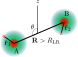
\includegraphics[width=\textwidth]{interaccionRR}
\end{minipage}
\hspace{5mm}
\begin{minipage}[c]{0.4\textwidth}
\centering
\caption{\label{fig:interaccionRR}Sistema de dos átomos de Rydberg cuyo eje interatómico está a un ángulo $\theta$ respecto al eje de cuantización. Las posiciones de los electrones de Rydberg son $\hat{\vektor{r}}_\sm{1}$ y $\hat{\vektor{r}}_\sm{2}$. La distancia interatómica es más grande que el radio de Le Roy $R_\sm{\text{LR}}$, de forma que las funciones de onda electrónicas no se solapen.}
\end{minipage}
\end{figure}

$\hat{\iH}_\sm{0}$ es el hamiltoniano de los estados de Rydberg no perturbados, $\hat{\iH}_\sm{\text{int}}$ engloba la interacción electrostática entre ambos electrones Rydberg, entre ambos núcleos y entre el electrón Rydberg de un átomo con el núcleo del otro átomo.

\p En el marco de esta aproximación, el vector $\vektor{R}$ se trata como un parámetro y no como operador, además su dirección $\vektor{n}$ se toma respecto al eje de cuantización, por lo que es posible escoger un marco donde $\vektor{n}$ se encuentre a un ángulo polar $\theta$ y un ángulo azimutal $\varphi=0$ respecto al eje de cuantización. Tomando en cuenta los términos de estructura fina se tiene que $\hat{\iH}_\sm{0}=\hat{\iH}_\sm{0;1}\otimes\hat{\mathbb{I}}_\sm{2}+\hat{\mathbb{I}}_\sm{1}\otimes\hat{\iH}_\sm{0;2}$ donde

\begin{equation}
\label{ec:hamiltonianoNoPerturbado}
\hat{\iH}_\sm{0;i}=\frac{\hat{\vektor{P}}_\sm{i}^{2}}{2m_\sm{e}}+V(r_\sm{i})-\frac{\hat{\vektor{P}}_\sm{i}^{4}}{8m_\sm{e}^{3}c^{2}}+\left(\frac{Z_\sm{i}e^{2}}{4\pi\epsilon_\sm{0}}\right)\frac{g_\sm{s}}{4m_\sm{e}^{2}c^{2}}\frac{1}{r_\sm{i}^{3}}\hat{\vektor{L}}_\sm{i}\cdot\hat{\vektor{S}}_\sm{i}+\left(\frac{Z_\sm{i}e^{2}}{4\pi\epsilon_\sm{0}}\right)\frac{\pi\hbar^{2}}{2m_\sm{e}^{2}c^{2}}\delta(\hat{\vektor{r}}_\sm{i}),
\end{equation}

con $g_\sm{s}$ el factor de Landé. Los valores valores propios de energía entonces son, hasta primer orden

\begin{equation}
\label{ec:energiaNoPerturnado}
\E_\sm{n,j;i}^{[1]}=-\frac{hcR_\sm{i}^{*}}{n^{2}}\left[1+\frac{(Z_\sm{i}\alpha)^{2}}{n(j+1/2)}-\frac{3(Z_\sm{i}\alpha)^{2}}{4n^{2}}\right],
\end{equation}

y $\alpha$ la constante de estructura fina. Como están involucrados dos átomos, una opción sensata para describir el sistema es utilizar una base construida como el producto tensorial de las bases atómicas individuales $\ket{n_\sm{1}l_\sm{1}j_\sm{1}m_\sm{1};n_\sm{2}l_\sm{2}j_\sm{2}m_\sm{2}}$, donde se hace la omisión usual de los números cuánticos de espín $s_\sm{1}=s_\sm{2}=1/2$ en la notación. De esta forma, cuando $R\to\infty$ la energía de un estado del sistema es simplemente la suma de las energías de átomos individuales, dadas por la ecuación~\ref{ec:energiaNoPerturnado}. Sin embargo, para distancias $R$ lo bastante cercanas, la interacción entre los átomos cambia esto.

\p Si el sistema de referencia se coloca en el núcleo A del primer átomo (figura~\ref{fig:interaccionRR}), y además la distancia interatómica $R$ es suficientemente grande para asegurar que las funciones de onda electrónicas no se solapen, entonces el hamiltoniano de interacción es

\begin{equation}
\label{ec:hamiltonianoInteraccionRydberg}
\hat{\iH}_\sm{\text{int}}(\vektor{R})=\frac{e^{2}}{4\pi\epsilon_\sm{0}}\left(\frac{Z_\sm{1}Z_\sm{2}}{\norm{\vektor{R}}}-\frac{Z_\sm{2}}{\norm{\vektor{R}-\hat{\vektor{r}}_\sm{1}}}-\frac{Z_\sm{1}}{\norm{\vektor{R}+\hat{\vektor{r}}_\sm{2}}}+\frac{1}{\norm{\vektor{R}+\hat{\vektor{r}}_\sm{2}-\hat{\vektor{r}}_\sm{1}}}\right),
\end{equation}

para $R>R_\sm{\text{LR}}$ y donde $R_\sm{\text{LR}}=2\left(\sqrt{\braket{\hat{r}^{2}}_\sm{1}}+\sqrt{\braket{\hat{r}^{2}}_\sm{2}}\right)$ es el \emph{radio de Le Roy}. Al utilizar la base esférica $\vektor{e}_\sm{\pm}=\mp\left(\vektor{e}_\sm{x}\mp i\vektor{e}_\sm{y}\right)/\sqrt{2}$ y $\vektor{e}_\sm{0}=\vektor{e}_\sm{z}$, el hamiltoniano de interacción~\ref{ec:hamiltonianoInteraccion} se puede expresar en su expansión multipolar

\begin{equation}
\label{ec:expansionMultipolar}
\hat{\iH}_\sm{\text{int}}(\vektor{R})=\frac{1}{4\pi\epsilon_\sm{0}}\left[\frac{(1-Z_\sm{1})(1-Z_\sm{2})e^{2}}{R}+\sum_{\kappa=1}^{\infty}\frac{V_\sm{\kappa}}{R^{\kappa+1}}+\sqrt{4\pi}\sum_{\kappa_{1},\kappa_{2}=1}^{\infty}\frac{V_\sm{\kappa_{1},\kappa_{2}}}{R^{\kappa_{1}+\kappa_{2}+1}}\right],
\end{equation}

en donde

\begin{equation}
\label{ec:vectorPotencial}
V_\sm{\kappa}=\sum_{q=-\kappa}^{\kappa}Y_\sm{\kappa,q}^{*}(\vektor{n})\sum_{j=1}^{2}(-1)^{j\kappa}(1-Z_\sm{j})\hat{p}_\sm{\kappa,q}^{(3-j)},
\end{equation}

\begin{equation}
\label{ec:matrizPotencial}
V_\sm{\kappa_{1},\kappa_{2}}=(-1)^{\kappa_{2}}\sum_{q_{1}=-\kappa_{1}}^{\kappa_{1}}\sum_{q_{2}=-\kappa_{2}}^{\kappa_{2}}\frac{Y_\sm{\kappa_{1}+\kappa_{2},q_{1}+q_{2}}^{*}(\vektor{n})}{\sqrt{2(\kappa
_{1}+\kappa_{2})+1}}\sqrt{\binom{\kappa_{1}+\kappa_{2}-q_{1}-q_{2}}{\kappa_{1}-q_{1}}\binom{\kappa_{1}+\kappa_{2}+q_{1}+q_{2}}{\kappa_{2}+q_{2}}}\hat{p}_\sm{\kappa_{1},q_{1}}^{(1)}\hat{p}_\sm{\kappa_{2},q_{2}}^{(2)},
\end{equation}

con $\hat{p}_\sm{\kappa,q}^{(i)}$ los \emph{operadores multipolares esféricos}, dados por

\begin{equation}
\label{ec:operadorMultipolarEsferico}
\hat{p}_\sm{\kappa,q}^{(i)}=e\hat{r}_\sm{i}^{\kappa}\sqrt{\frac{4\pi}{2\kappa+1}}Y_\sm{\kappa,q}(\hat{\vektor{n}}_\sm{i}),
\end{equation}

y $\hat{\vektor{n}}_\sm{i}=(\hat{\theta}_\sm{i},\hat{\varphi}_\sm{i})$ es el operador dirección de $\hat{\vektor{r}}_\sm{i}$.

\p Retomando el caso de átomos alcalinos tenemos $Z_\sm{1}=Z_\sm{2}=1$, por lo cual $V_\sm{\kappa}=0$ para todo valor de $\kappa$. De esta forma, los primeros dos términos de la ecuación~\ref{ec:expansionMultipolar} se anulan:

\begin{equation}
\label{ec:expansionMultipolarAlcalinos}
\hat{\iH}_\sm{\text{int}}(\vektor{R})=\frac{\sqrt{4\pi}}{4\pi\epsilon_\sm{0}}\sum_{\kappa_{1},\kappa_{2}=1}^{\infty}\frac{V_\sm{\kappa_{1},\kappa_{2}}}{R^{\kappa_{1}+\kappa_{2}+1}}.
\end{equation}

Observamos que el hamiltoniano de interacción anterior es una expansión en serie en potencias $\varrho=\kappa_{1}+\kappa_{2}+1$ del inverso de la distancia interatómica. Esta expansión empieza por $\varrho=3$, por lo tanto la contribución de menor orden es la interacción dipolo-dipolo, la cual exhibe la carga neutra de los átomos de Rydberg.

\subsection{\label{sub:intensidadInteraccion}Intensidad de interacción}

Si bien varios experimentos han investigado términos de interacción de orden superior, nosotros restringimos la discusión al término de menor orden, la interacción dipolo-dipolo. En este límite, el hamiltoniano de interacción adopta la forma usual

\begin{equation}
\label{ec:interaccionDipoloDipolo}
\hat{\iH}_\sm{\text{int}}(\vektor{R})=\frac{\hat{\vektor{d}}_\sm{1}\cdot\hat{\vektor{d}}_\sm{2}-3(\vektor{n}\cdot\hat{\vektor{d}}_\sm{1})(\vektor{n}\cdot\hat{\vektor{d}}_\sm{2})}{R^{3}}\eqqcolon\hat{\iH}_\sm{\text{dd}}(\vektor{R}),
\end{equation}

donde $\hat{\vektor{d}}_\sm{i}=e\hat{\vektor{r}}_\sm{i}$. Podemos estudiar este hamiltoniano en dos regímenes, distancias interatómicas pequeñas o grandes, que da lugar a una dependencia $1/R^{3}$ o $1/R^{6}$ en la interacción como se detalla a continuación.

\subsubsection{\label{ssub:resonanciaForster}Intensidad dipolo-dipolo y resonancias de Förster}

La representación en la base esférica del hamiltoniano anterior (ec.~\ref{ec:interaccionDipoloDipolo}) se puede encontrar directamente utilizando $\hat{d}_\sm{j,\pm}=\mp\left(\vektor{d}_\sm{j,x}\pm i\vektor{d}_\sm{j,y}\right)/\sqrt{2}$, o utilizando la expansión~\ref{ec:expansionMultipolarAlcalinos} con $\kappa_\sm{1}=\kappa_\sm{2}=1$. De esta forma, si compactamos la notación como $\ket{1;2}=\ket*{n_\sm{1}l_\sm{1}j_\sm{1}m_\sm{1};n_\sm{2}l_\sm{2}j_\sm{2}m_\sm{2}}$, tenemos que

\begin{equation}
\label{ec:fuerzaDipoloDipolo}
\braket{\hat{\iH}_\sm{\text{dd}}(\vektor{R})}=\braket{1;2|\hat{\iH}_\sm{\text{dd}}(\vektor{R})|1';2'}=\frac{C_\sm{3}(\theta)}{R^{3}},
\end{equation}

siendo $C_{3}(\theta)$ una suma de productos de elementos de matriz radiales y elementos de matriz angulares de ambos átomos del Hamiltoniano total (ec.~\ref{ec:hamiltonianoDosAtomos})~\cite{paris} por factores angulares que provienen del armónico esférico {\color{purple}$Y_\sm{2,q_{1}+q_{2}}^{*}(\vektor{n})=Y_\sm{2,q_{1}+q_{2}} (\theta,0)$} de la ecuación~\ref{ec:matrizPotencial}. La ecuación~\ref{ec:fuerzaDipoloDipolo} representa la intensidad de la interacción entre los átomos de Rydberg, la cual es de tipo dipolo-dipolo debido a la potencia cúbica del inverso de la distancia interatómica.

\p El hamiltoniano dipolo-dipolo $\hat{\iH}_\sm{\text{dd}}$ proporciona el acoplamiento entre diferentes \emph{estados producto} $\ket{1;2}$ y $\ket{1';2'}$, la parte atómica $\hat{\iH}_\sm{0}$ del sistema determina la diferencia de energía inicial $h\Delta_\sm{\text{F}}$ entre dichos estados producto como se muestra en la figura~\ref{fig:defectoForster}; a esta diferencia de energía se le llama \emph{defecto de Förster}. Aun cuando la separación de los niveles de energía para cada átomo ($h\Delta_\sm{1}$ y $h\Delta_\sm{2}$) pueda ser diferente, pueden resultar que el valor del defecto de Förster en la base de estados producto sea pequeño. Si se da tal (casi) resonancia, los niveles involucrados constituyen la contribución dominante de la interacción dipolo-dipolo~\cite{paris}. Así pues, la representación matricial del hamiltoniano, de dimensión infinita, se aproxima por una matriz pequeña donde sólo se involucran estados producto casi resonantes.

\begin{figure}
\centering
\begin{minipage}{0.8\textwidth}
\centering
\includegraphics[width=0.7\textwidth]{defectoForster}
\caption[Defecto Föster]{\label{fig:defectoForster}La estructura de niveles de dos átomos de Rydberg, preparados en $\ket{1}$ y $\ket{2}$, modifica la intensidad de interacción entre estos debido al acoplamiento dipolar a otros estados $\ket{1'}$ y $\ket{2'}$. La interacción se maximiza para defectos de Förster pequeños. Imagen reproducida de~\cite{paris}.}
\end{minipage}
\end{figure}

Las conocidas \emph{resonancias de Förster} ocurren cuando la energía de dos estados producto es degenerada ($\Delta_\sm{\text{F}}=0$), la cual resulta en un acoplamiento resonante entre los estados que conduce a una dependencia \scalebox{0.9}[1]{$\sim$}$1/R^{3}$ de la interacción. En la práctica se habla de resonancias de Förster aun cuando los estados pareja no sean exactamente resonantes, como en el rubidio con los estados pareja $\ket*{41\mathrm{D};49\mathrm{S}}$ y $\ket*{42\mathrm{P};49\mathrm{P}}$~\cite{comparat}.

\subsubsection{\label{ssub:vanderWaals}Fuerza de interacción de van der Waals}

En el caso de que el defecto cuántico sea grande comparado con la intensidad de la interacción $\abs{h\Delta_\sm{\text{F}}}\gg\abs{C_\sm{3}(\theta)/R^{3}}$ (distancias interatómicas grandes), el hamiltoniano de acoplamiento dipolo-dipolo $\hat{\iH}_\sm{\text{dd}}(\vektor{R})$ se puede entender como una perturbación. Es necesario abordar la teoría de perturbaciones a segundo orden, pues la corrección a primer orden de los niveles de energía es

\begin{equation}
\label{ec:perturbacionPrimerOrden}
\Delta\E=\braket*{n_\sm{1}l_\sm{1}j_\sm{1}m_\sm{1};n_\sm{2}l_\sm{2}j_\sm{2}m_\sm{2}|\hat{\iH}_\sm{\text{dd}}(\vektor{R})|n_\sm{1}l_\sm{1}j_\sm{1}m_\sm{1};n_\sm{2}l_\sm{2}j_\sm{2}m_\sm{2}},
\end{equation}

como el operador dipolar $\hat{\vektor{d}}$ no acopla estados de la misma paridad, lo anterior es cero. A segundo orden, la corrección en la energía es

\begin{equation}
\label{ec:perturbacionSegundoOrden}
\Delta\E=\sum_{i,k}\frac{\abs{\braket*{n_\sm{i}l_\sm{i}j_\sm{i}m_\sm{i};n_\sm{k}l_\sm{k}j_\sm{k}m_\sm{k}|\hat{\iH}_\sm{\text{dd}}(\vektor{R})|n_\sm{1}l_\sm{1}j_\sm{1}m_\sm{1};n_\sm{2}l_\sm{2}j_\sm{2}m_\sm{2}}}^{2}}{\E_\sm{1,2}-\E_\sm{i,k}}.
\end{equation}

Observando que el hamiltoniano en la ecuación~\ref{ec:interaccionDipoloDipolo} va como $1/R^{3}$, este término puede salir del valor esperado y la suma en la ecuación de arriba queda

\begin{equation}
\label{ec:fuerzavanderWaals}
\Delta\E=\frac{C_\sm{6}(\theta)}{R^{6}},
\end{equation}

ergo a largas distancias se tiene una interacción de \emph{van der Waals}.

\begin{figure}
\centering
\begin{minipage}{0.8\textwidth}
\centering
\includegraphics[width=0.8\textwidth]{intensidadInteraccion}
\caption{\label{fig:intensidadInteraccion}Intensidad de interacción de dos átomos de Rb en estado base, dos átomos de Rb excitados en $\text{100}\mathrm{S}$ y iones. Imagen reproducida de~\cite{saffman}.}
\end{minipage}
\end{figure}

\subsection{\label{sub:bloqueoRydberg}Bloqueo de Rydberg}

Los elementos de matriz para el hamiltoniano de interacción entre dos átomos están dados en~\ref{sub:intensidadInteraccion}, además de que la parte atómica del hamiltoniano completo proporciona el defecto Förster. En la base de estados producto $\{\ket{1;2},\ket{1';2'}\}$, el hamiltoniano del sistema de dos átomos neutros~\ref{ec:hamiltonianoDosAtomos} queda representado por

\begin{equation}
\label{ec:hamiltonianoCompleto}
\hat{\iH}(\vektor{R})=\begin{pmatrix}
0 & \dfrac{C_\sm{3}}{R^{3}}\\[6mm]
\dfrac{C_\sm{3}}{R^{3}} & \hbar\Delta_\sm{\text{F}}
\end{pmatrix},
\end{equation}

donde $\Delta_\sm{\text{F}}=\Delta_\sm{1}+\Delta_\sm{2}$~(figura~\ref{fig:defectoForster}). La representación matricial anterior es para el caso en el que se define como 0 la energía del estado $\ket{1;2}$, cuyos valores propios de energía son

\begin{equation}
\label{ec:energiasPropias}
\E_\sm{\pm}=\frac{\hbar\Delta_\sm{\text{F}}}{2}\pm\sqrt{\left(\frac{\hbar\Delta_\sm{\text{F}}}{2}\right)^{2}+\left(\frac{C_\sm{3}}{R^{3}}\right)^{2}}.
\end{equation}

Si los átomos no interactúan, la diferencia de energía entre los estados $\ket{1';2'}$ y $\ket{1;2}$ será $\Delta\E_\sm{0}=\hbar\Delta_\sm{\text{F}}$. La interacción dipolo-dipolo entre los átomos modifica la energía de estos estados, que ahora depende de la separación entre los átomos (ec.~\ref{ec:energiasPropias}). La diferencia de energía entre los estados es

\begin{equation}
\label{ec:diferenciaEnergia}
\Delta\E=\E_\sm{+}-\E_\sm{-}=2\sqrt{\left(\frac{\hbar\Delta_\sm{\text{F}}}{2}\right)^{2}+\left(\frac{C_\sm{3}}{R^{3}}\right)^{2}},
\end{equation}

si la interacción es intensa (distancias interatómicas cortas), entonces $\abs{h\Delta_\sm{\text{F}}}\ll\abs{C_\sm{3}(\theta)/R^{3}}$ y los niveles de energía se separan, respecto al caso sin interacción, por

\begin{equation}
\label{ec:diferenciaEnergiasCercano}
\Delta\E_\sm{\text{b}}\coloneqq\Delta\E-\Delta\E_\sm{0}=\frac{2\abs{C_\sm{3}}}{R^{3}},
\end{equation}

mientras que para interacciones débiles $\abs{h\Delta_\sm{\text{F}}}\gg\abs{C_\sm{3}(\theta)/R^{3}}$ (distancias interatómicas grandes), se obtiene

\begin{equation}
\label{ec:diferenciaEnergiasLejano}
\Delta\E_\sm{\text{b}}=\frac{2\abs{C_\sm{3}}^{2}}{\hbar\abs{\Delta_{\text{F}}}R^{6}}=\frac{2C_\sm{6}}{R^{6}}.
\end{equation}

Por supuesto, ambas expresiones deben conciliarse para una distancia intermedia, misma que algunas veces la llaman \emph{radio de van der Waals}. Igualando ambas expresiones~\ref{ec:diferenciaEnergiasCercano} y \ref{ec:diferenciaEnergiasLejano} se concluye que

\begin{equation}
\label{ec:radiovanderWaals}
R_\sm{\text{vdW}}=\sqrt[3]{\frac{\abs{C_{3}}}{\hbar\abs{\Delta_{\text{F}}}}}=\sqrt[6]{\frac{C_{6}}{\hbar\abs{\Delta_{\text{F}}}}}.
\end{equation}

En resumen, la energía de interacción entre dos átomos de Rydberg muestra una fuerte dependencia en el número cuántico principal efectivo $n^{*}$ $\bigl($pues $C_\sm{3}\propto (n^{*})^{4}$, $\Delta_\sm{\text{F}}\propto (n^{*})^{-3}$ y $C_\sm{6}\propto (n^{*})^{11}\bigr)$.

\p En la figura~\ref{fig:bloqueoRydberg} se muestra el cambio de energía del nivel asociado al estado $\ket{1';2'}$ respecto al nivel correspondiente al estado $\ket{1;2}$. Este fenómeno se denomina \emph{bloqueo de Rydberg}, pues aún teniendo dos láseres resonantes con las transiciones de los átomos individuales (uno resonante con $\ket{1}\leftrightarrow\ket{1'}$ y el otro con $\ket{2}\leftrightarrow\ket{2'}$), el cambio de energía debido a la interacción dipolar deja fuera de resonancia el estado $\ket{1',2'}$, siempre y cuando el ancho de línea de la excitación sea más pequeño que el potencial de interacción $2\abs{C_\sm{\beta}}/R^{\beta}$.

\begin{figure}
\centering
\begin{minipage}{0.8\textwidth}
\centering
\includegraphics[width=0.4\textwidth]{bloqueoRydberg}
\caption[Bloqueo de Rydberg]{\label{fig:bloqueoRydberg}Principio del bloqueo de Rydberg entre dos átomos separados una distancia $R$. Cuando los átomos están en el estado $\ket{1';2'}$ interactúan fuertemente, lo cual conduce a un desplazamiento de energía $\Delta\E_\sm{\text{b}}$. Cuando este desplazamiento se hace más grande que $\hbar\Omega_\sm{2}$, el láser queda fuera de resonancia con la transición que acopla el estado de excitación simple con el de excitación doble, y sólo un átomo se puede transferir a un estado de Rydberg a la vez.}
\end{minipage}
\end{figure}

\section{\label{sec:opticaCuantinaNoLineal}Óptica Cuántica no lineal}

El estudio en Óptica es el uso de la materia para manipular a la luz, alterar sus características o propiedades, lo más conocido es el cambio en la amplitud y fase de la luz debido al medio. La interacción se puede exponer de varias maneras, de forma semiclásica como lo describimos en~\ref{sub:atomo3Niveles} y cuyo enfoque es microscópico (descripción de la dinámica de un solo átomo inmerso en un campo de radiación clásico); también está la descripción macroscópica donde consideramos al medio como un todo, sus propiedades son el resultado conjunto de las propiedades de sus constituyentes. Como ya vimos en~\ref{sub:eit}, una de estas propiedades es la polarización $P$ del medio, definida como el momento dipolar promedio por unidad de volumen y que es la respuesta del medio a campos eléctricos externos:

\begin{equation}
\label{ec:polarizacion}
P(t)=\epsilon_\sm{0}\sum_{k\geq1}\chi^{(k)}E^{k}(t),
\end{equation}

donde $\chi^{(k)}$ son las susceptibilidades eléctricas, las cuales dependen completamente del medio. Cuando el valor de $\chi^{(k>1)}$ es despreciable comparado con $\chi^{(1)}$ decimos que el medio es lineal, en caso contrario alguna de las susceptibilidades de orden superior del medio es comparable o mayor a $\chi^{(1)}$ y, por ende, su respuesta es proporcional a alguna potencia del campo eléctrico, lo cual nombramos \emph{Óptica no lineal}~\cite{boyd}. Es posible inducir no linealidades en un medio empleando haces de luz de alta potencia, lo cual es inconveniente en nuestro caso puesto que queremos hacer experimentos a muy bajas intensidades, incluso al nivel de unos cuantos fotones.

\p La \emph{Óptica Cuántica no lineal} se encarga de estudiar la luz y como controlarla usando medios cuyo comportamiento no lineal depende del número de fotones. Las altas no linealidades provocan que la luz interactúe consigo misma, un comportamiento que no sucede normalmente, esto nos provee de mecanismos para crear estados no clásicos de luz~\cite{peyronel,kumlin}.

\subsection{\label{sub:opticaCuanticaNoLinealRydberg}Óptica Cuántica no lineal de Rydberg}

Buscamos convertir pulsos de luz coherente de pocos fotones en luz no clásica mediante el uso de estados de Rydberg, lo que se nombra como \emph{Óptica Cuántica no lineal de Rydberg}~\cite{firstenberg1}. El bloqueo de Rydberg junto con EIT forman una pareja interesante de fenómenos para producir altas no linealidades en un medio atómico, por ejemplo, realizar EIT donde el segundo estado excitado es uno de Rydberg: lejos de resonancia del haz de prueba el medio es opaco, conforme la frecuencia de este láser se hace resonante ingresaremos a la ventana de transparencia de EIT, pero también comenzarán a excitarse los estados de Rydberg generando zonas de bloqueo donde se rompe la condición de EIT. Gracias al bloqueo de Rydberg, un solo fotón altera la dinámica de miles de átomos.

\p Fue a inicios de este milenio cuando surge la idea de utilizar los átomos de Rydberg para crear estados no clásicos de luz~\cite{lukin2}, hecho que reavivo el interés por los átomos de Rydberg. En 2007 se incorpora el fenómeno de EIT para observar la dinámica coherente entre la luz y los átomos~\cite{mohapatra}, evitando la detección destructiva del sistema. Luego se impulsó el uso de átomos de Rydberg para controlar la luz a escala de fotones individuales~\cite{dudin,peyronel,maxwell}.

\p Los fotones, al viajar a través de estos medios no lineales, dan lugar a \emph{polaritones}, una cuasipartícula que es la superposición de una excitación material y radiación electromagnética. Al emplear átomos de Rydberg, su fuerte interacción dipolo-dipolo $\bigl(\alpha_\sm{E}\propto(n^{*})^{7}\text{ y }C_\sm{6}\propto(n^{*})^{11}\bigr.$~tabla~\ref{tab:propiedadesRydberg}$\bigl.\bigr)$ se mapea a los fotones, dicho de otra forma, la componente material de los polaritones dota a estas cuasipartículas la capacidad de interactuar del medio. El estudio de esta interacción de fotones es interesante y se ha utilizado, por ejemplo, para hacer a los fotones atractivos~\cite{firstenberg2} o fotones repulsivos~\cite{cantu}; estos estados de luz claramente son no clásicos puesto que la luz no exhibe estos comportamientos en las teorías clásicas.

\section{\label{sec:rubidio}Rubidio}

La especie atómica que utilizamos es el rubidio (Rb), que al ser un metal alcalino ofrece facilidades en la producción de átomos de Rydberg dada la cantidad de teoría y métodos desarrollados para este tipo de sistemas y su interacción con luz láser. No utilizamos hidrógeno (H) puesto que la transición del estado base al primer estado excitado es ultravioleta, esa misma transición es accesible en el litio Li pero del primer estado excitado a uno de Rydberg es nuevamente ultravioleta; existen técnicas, la tecnología y óptica para esas longitudes de onda, sin embargo, llevar a cabo experimentos de esa naturaleza es más complicado y excesivamente costoso.

\p Los átomos de Rb y cesio Cs son los que poseen transiciones a estados de Rydberg muy accesibles (en el visible), elegimos rubidio por motivos prácticos. En la naturaleza existen dos isótopos del rubidio, a saber $\prescript{85}{}{\mathrm{Rb}}$ y $\prescript{87}{}{\mathrm{Rb}}$, gran parte de sus propiedades físicas son bien conocidas y se resumen en las hojas de datos de Steck~\cite{rb85,rb87}. Tomando en cuenta la estructura fina el estado base del Rb es $5\prescript{2}{}{\mathrm{S}}_\sm{1/2}$ y el primer estado excitado está desdoblado en $5\prescript{2}{}{\mathrm{P}}_\sm{1/2}$ y $5\prescript{2}{}{\mathrm{P}}_\sm{3/2}$ gracias al acoplamiento espín-órbita; la transición $5\prescript{2}{}{\mathrm{S}}_\sm{1/2}\to5\prescript{2}{}{\mathrm{P}}_\sm{1/2}$ ($5\prescript{2}{}{\mathrm{S}}_\sm{1/2}\to5\prescript{2}{}{\mathrm{P}}_\sm{3/2}$) se llama \emph{transición/línea D1} (\emph{transición/línea D2}).

\p La excitación del Rb a otros niveles de energía debe de seguir las reglas de selección de estas transiciones:

 \begin{equation}
\label{ec:reglasSeleccion}
\begin{split}
\Delta L= & \pm1\\
\Delta J= & \hspace{1mm}0,\pm1\\
\Delta F= & \hspace{1mm}0,\pm1\\
\Delta M_\sm{F}= & \hspace{1mm}0,\pm1\\
\Delta F\neq0\text{ si }M_\sm{F}\hspace{0.5mm} & =M_\sm{F'}=0.
\end{split}
\end{equation}

Son estas reglas de selección a partir de las cuales se tienen las líneas D1 y D2. Las dos formas más utilizadas para obtener estados de Rydberg con Rb son:

\begin{equation}
\label{ec:rydbergRb1}
5\mathrm{S}\xrightarrow[]{\SI{780}{\nano\meter}}5\mathrm{P}\xrightarrow[]{\SI{480}{\nano\meter}}n\mathrm{S}/n\mathrm{D},
\end{equation}

\begin{equation}
\label{ec:rydbergRb2}
5\mathrm{S}\xrightarrow[]{\SI{420}{\nano\meter}}6\mathrm{P}\xrightarrow[]{\SI{1016}{\nano\meter}}n\mathrm{S}/n\mathrm{D},
\end{equation}

cuyas frecuencias son del visible o infrarrojo, disponibles con láseres comerciales de diodo cuyo costo es mucho menor que láseres ultravioletas.

\section{\label{sec:laboratorioOCR}Labortatorio de Óptica Cuántica de Rydberg}

El proyecto de doctorado lo llevaré a cabo en el laboratorio de Óptica Cuántica de Rydberg a cargo del Dr. Asaf Paris Mandoki. La meta del laboratorio es realizar y estudiar experimentos de óptica cuántica no lineal con el uso de átomos de Rydberg con la visión de ampliar el conocimiento en interacciones fundamentales entre luz y materia.

\begin{figure}[H]
\centering
\begin{minipage}{0.8\textwidth}
\centering
\includegraphics[width=0.725\textwidth]{sistemaLaseres}
\caption{\label{fig:sistemaLaseres}Sistema actual de láseres para enfriar y atrapar átomos, así como producir átomos de Rydberg. En la mesa óptica se encuentran el láser maestro que es la referencia en frecuencia de los láseres de enfriamiento, rebombeo e imagen. También está el láser azul para las transiciones a estados de Rydberg.}
\end{minipage}
\end{figure}

El surgimiento del laboratorio comenzó en el 2018, durante ese año y el siguiente se realizó el montaje y construcción del sistema de láseres, mismo que sirve para la generación de la luz que es necesaria para efectuar los experimentos deseados. Este sistema ha ido creciendo y crecerá con el tiempo por los requerimientos de los experimentos, a día de hoy el sistema de láseres está conformado de un láser maestro de luz infrarroja ($\SI{780}{\nano\meter}$) anclado en frecuencia a una cavidad de ultra baja expansión (ULE por sus siglas en inglés) con el método de Pound–Drever–Hall~\cite{black} (PDH), sirve de referencia para anclar otros tres láseres: enfriamiento y rebombeo, utilizados para enfriar la nube de átomos (una trampa magneto-óptica, MOT por sus siglas en inglés) y el láser de imagen para obtener información del medio atómico.

\p Otro láser del sistema es el de $\SI{960}{\nano\meter}$, anclado de igual forma a la cavidad mediante PDH, se utiliza para realizar las transiciones del primer estado excitado a un estado superior (ver~\ref{sub:atomo3Niveles}). Se planea instalar un láser de $\SI{1064}{\nano\meter}$ para una trampa dipolar con la cual aumentaremos el número de átomos que se atrapan en la MOT y la densidad de dicho ensamble.

\p Luego, a partir del año 2020 fuimos construyendo el sistema de vacío, así como el montaje optomecánico y de bobinas para la implementación de la MOT~\cite{alonso}. Las condiciones alcanzadas con el vacío, después del proceso de horneado, bombeo y optimización, son una presión interna por debajo de lo $\SI{10e-10}{\milli\bar}$ y temperaturas inferiores a los $\SI{100}{\micro\kelvin}$ del conjunto de átomos atrapados. El sistema de láseres y de vacío nos permitió generar átomos de Rydberg que detectamos con la Transparencia Electromagnéticamente Inducida (fig.~\ref{fig:eit}).

\newsavebox{\avancesBox}
\begin{figure}[!ht]
\centering
\begin{minipage}{0.9\textwidth}
\centering
\sbox{\avancesBox}{\includegraphics[width=0.5\linewidth]{sistemaVacio}}
\subcaptionbox{\label{fig:vacioActual}}[0.45\linewidth]{
\vbox to \ht\avancesBox{
\vfill
\includegraphics[width=\linewidth]{eitExp}
\vfill}}
\hfill
\subcaptionbox{\label{fig:eit}}[0.5\linewidth]{\usebox{\avancesBox}}
\caption[Trabajo en laboratorio de OCR]{\label{fig:eitVacioActual}(a) Medición de EIT en el laboratorio de OCR en un ensamble de átomos de $\prescript{87}{}{\mathrm{Rb}}$ aproximadamente a $\SI{100}{\micro\kelvin}$, el estado de Rydberg de dicha medición fue $28\mathrm{S}$. (b) Actualidad: sistema de vacío y optomecánica requerida para la MOT y los demás haces láser.}
\end{minipage}
\end{figure}